\begin{figure}[tb]
  \centering
  \begin{subfigure}{0.6\linewidth}
  \begin{subfigure}{1\linewidth}
    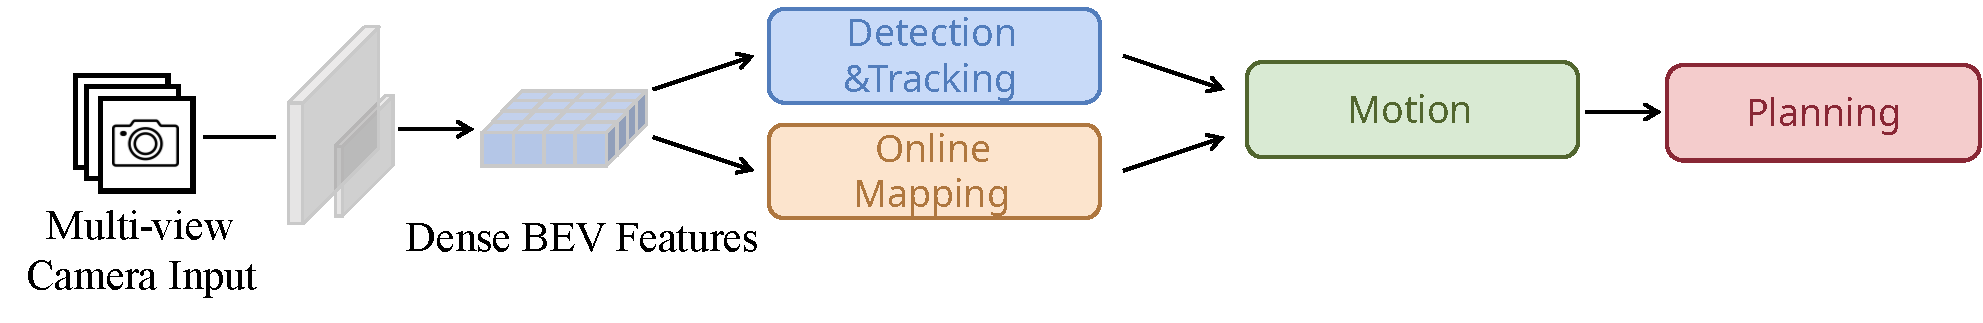
\includegraphics[width=1\linewidth]{Figures/pipeline_bev.pdf}
    \caption{BEV-Centric paradigm.}
    \label{fig:pipeline_bev}
  \end{subfigure}
  \hfill
  \\
  \begin{subfigure}{1\linewidth}
    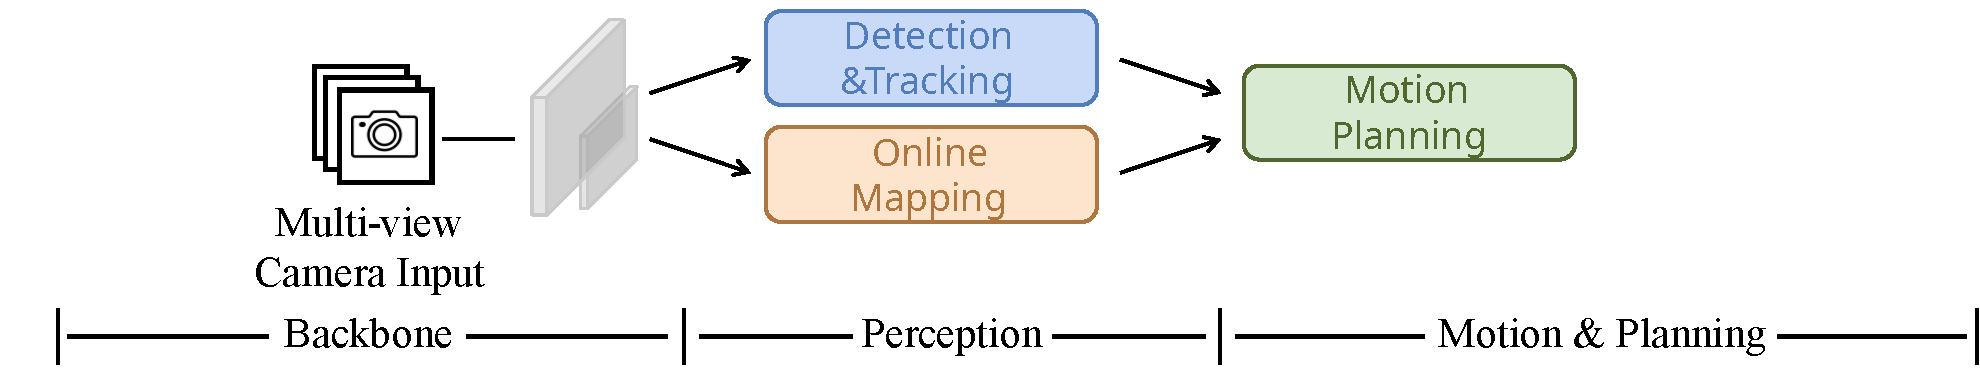
\includegraphics[width=1\linewidth]{Figures/pipeline_sparse.pdf}
    \caption{Sparse-Centric paradigm.}
    \label{fig:pipeline_sparse}
  \end{subfigure}
  \label{fig:short}
  \\
  \hfill
  \end{subfigure}
  \hspace{2pt}
  \begin{subfigure}{0.38\linewidth}
  \centering
    \begin{subfigure}{1\linewidth}
    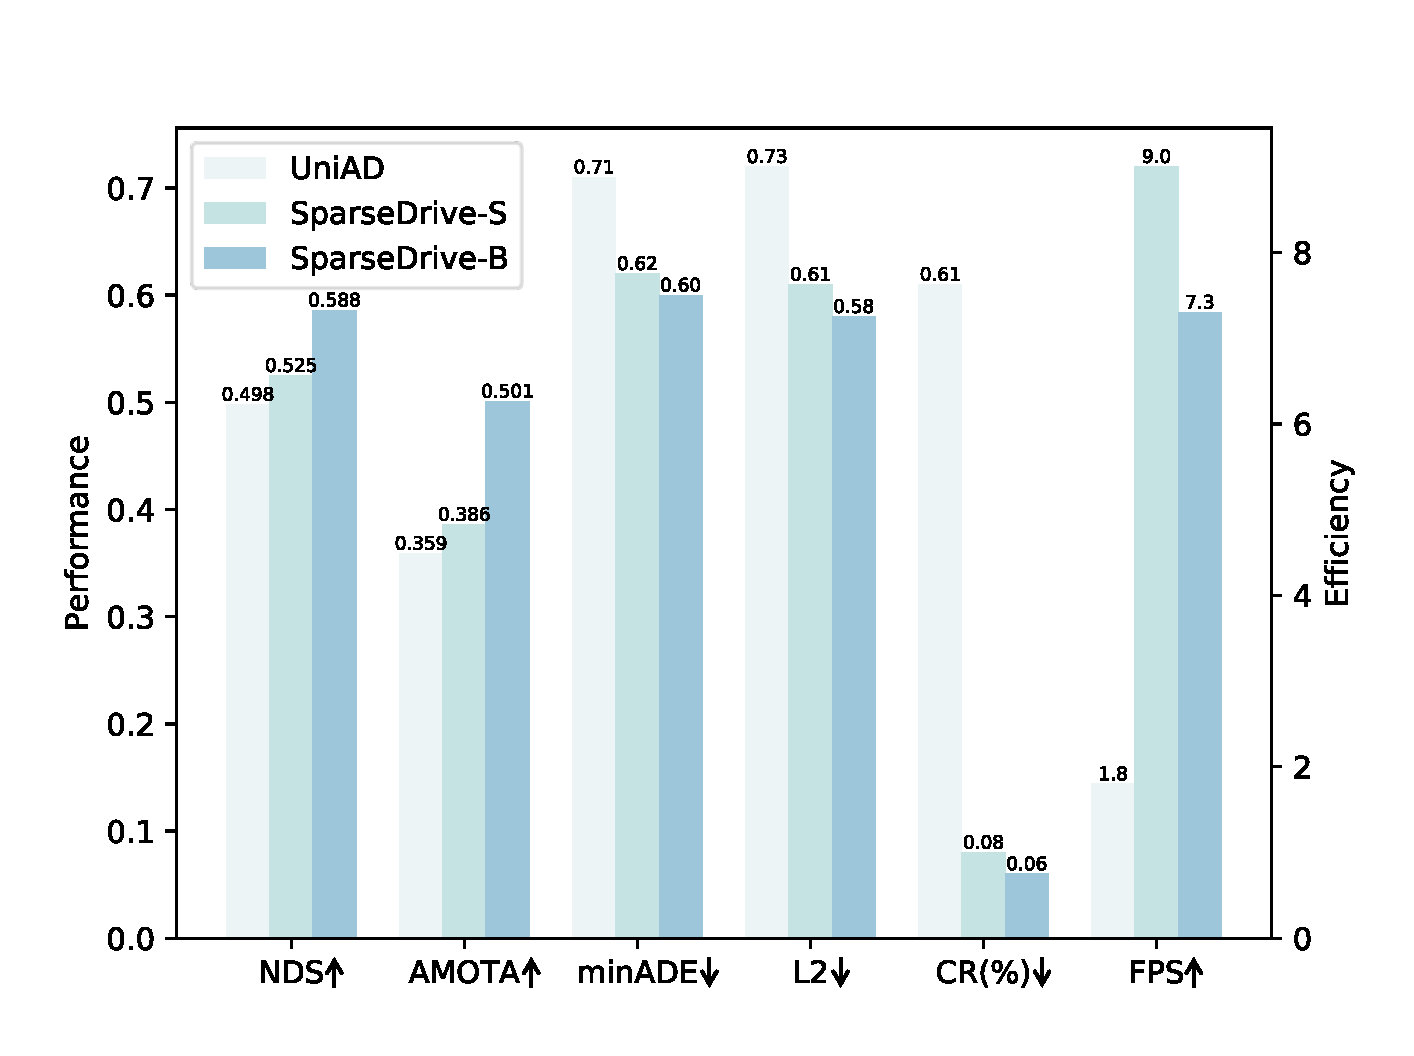
\includegraphics[width=1\linewidth]{Figures/comp.pdf}
    \caption{Comparison between our method and privous SOTA\cite{uniad}.}
    \label{fig:comp}
    \end{subfigure}
    \\
    \begin{subfigure}{1\linewidth}
    \end{subfigure}
    \\
    \begin{subfigure}{1\linewidth}
    \end{subfigure}

  \end{subfigure}
  
  \caption{The comparison of various end-to-end paradigms. (a) The BEV-Centric paradigm. (b) The proposed Sparse-Centric paradigm. (c) Performance and efficiency comparison between (a) and (b).}
  \label{fig:pipeline}
\end{figure}